% !TEX root = ../main.tex
\chapter{Principles of Spectroscopy}
\label{chapter_spectroscopy}
%-------------------------------------------------------------------------------
%	SECTION 1: INTRODUCTION TO SPECTROSCOPY
%-------------------------------------------------------------------------------

\section{Fundamentals of Spectroscopy}
\label{sec:spectroscopy_fundamentals}

\noindent Spectroscopy, in its broadest definition, is the study of the interaction between matter and electromagnetic radiation as a function of wavelength or frequency \cite{berman2011principleslaserspectroscopy, mukamel1995principlesnonlinearoptical}.
This technique provides insights into the composition, structure, and dynamics of physical systems by examining how they absorb, emit, or scatter light. The fundamental principle underlying all spectroscopic methods is that each atom, molecule, or complex system has a unique set of energy levels, and transitions between these levels involve the absorption or emission of photons with specific energies \todoref{find better source}\cite{boyd2008chapter1nonlinear}.

\subsection{Basic Principles}
\label{subsec:basic_principles}

\noindent The foundation of spectroscopy rests on the quantization of energy in atomic and molecular systems. According to quantum mechanics, atoms and molecules can exist only in discrete energy states \cite{albashetal2012quantumadiabaticmarkovian}. The energy difference between two states, $\Delta E$, determines the frequency $\nu$ or wavelength $\lambda$ of light that can be absorbed or emitted during a transition between these states, following Planck's relation:

\begin{equation}
	\Delta E = h\nu = \frac{hc}{\lambda}
	\label{eq:planck_relation}
\end{equation}

\noindent where $h$ is Planck's constant and $c$ is the speed of light. The energy structure of matter can thus be probed by observing the spectrum of absorbed or emitted radiation.
%-------------------------------------------------------------------------------
%   NEW SUBSECTION: CHARACTERIZATION OF ELECTROMAGNETIC RADIATION
%-------------------------------------------------------------------------------

\subsection{Characterization of Electromagnetic Radiation}
\label{subsec:em_radiation_characterization}

\noindent A monochromatic plane electromagnetic wave in free space (vacuum) can be written as
\begin{equation}
	E(\vec{r},t) = E_0 \cos(\vec{k} \cdot \vec{r} - \omega t + \phi)
	\label{eq:plane_wave}
\end{equation}
where $E_0$ is the (real) amplitude, $\phi$ a phase-kick, $\vec{k}$ the wavevector (spatial angular frequency), and $\omega$ the angular frequency of the wave.

The fundamental kinematic relations for propagation in vacuum are
\begin{equation}
	\omega = 2\pi\nu, \qquad |\vec{k}| = \frac{2\pi}{\lambda}, \qquad \lambda = \frac{c}{\nu} = \frac{2\pi c}{\omega}
	\label{eq:wavelength_frequency_relation}
\end{equation}
with $\nu$ the (cycle) frequency in hertz (Hz), $\lambda$ the wavelength. In a material medium the phase velocity is $v_p = c/n(\nu)$ and $\lambda$ is replaced by $\lambda_n = v_p/\nu = \lambda/n(\nu)$, where $n(\nu)$ is the refractive index.

\noindent Note that the \emph{magnitude of the wavevector } $k = 2\pi/\lambda$ (units m$^{-1}$), which appears explicitly in the plane wave phase $kz$ shall not be confused with the \emph{(spectroscopic) wavenumber} $\tilde{\nu}$, defined as
\begin{equation}
	\tilde{\nu} = \frac{1}{\lambda} \quad [\mathrm{cm}^{-1}].
	\label{eq:wavenumber_definition}
\end{equation}

The energetic content of radiation can be expressed equivalently to \eqref{eq:planck_relation} using any of the variables above:
\begin{equation}
	E = \hbar\omega = h c \, \tilde{\nu}
	\label{eq:energy_wavenumber_conversion}
\end{equation}
with $\hbar = h/2\pi$.

\todoidea{put this somewhere else}
\noindent Useful unit conversions (exact in the SI or by definition) frequently encountered in spectroscopy are:
\begin{align}
	1\,\mathrm{nm}      & = 10^{-9}\,\mathrm{m},                        &
	1\,\mu\mathrm{m}    & = 10^{-6}\,\mathrm{m},                        &
	1\,\mathrm{\AA}     & = 10^{-10}\,\mathrm{m},                         \\
	1\,\mathrm{cm}^{-1} & \approx 29.9792458\,\mathrm{GHz},             &
	1\,\mathrm{cm}^{-1} & \approx 1.23984198\times10^{-4}\,\mathrm{eV}.
	\label{eq:unit_conversions}
\end{align}
The gigahertz conversion uses $c = 2.99792458\times10^{10}\,\mathrm{cm\,s^{-1}}$; the electronvolt conversion uses Eq.~\eqref{eq:energy_wavenumber_conversion} and $1\,\mathrm{eV} = 1.602176634\times10^{-19}\,\mathrm{J}$.

%--- Spectral regions + energy dissipation addendum (Banwell) -----------------
\paragraph{Spectral Regions and Notation}
\noindent Spectral domains are commonly quoted in either wavelength $\lambda$ or wavenumber $\tilde{\nu}$ to avoid large powers of ten.
For example most electronic transitions occur in the visible range $\lambda \sim 400$--$750\,\mathrm{nm}$, which corresponds to $\tilde{\nu} \sim 13333$--$25000\,\mathrm{cm}^{-1}$. On the other hand, vibrational transitions, for example in a molecule typically occur in the infrared range $\lambda \sim 2.5$--$25\,\mu\mathrm{m}$, which corresponds to $\tilde{\nu} \sim 4000$--$400\,\mathrm{cm}^{-1}$.

\paragraph{Remark on Re-Emission}
\noindent Following absorption, isotropic spontaneous re-emission (radiative relaxation) redistributes photon directions so that only a negligible fraction re-enters the forward detection solid angle, yielding a net attenuation of the incident beam. The corresponding emission (fluorescence / phosphorescence) spectra, arising from these radiative pathways, will be exploited later in this work for extracting dynamical information from heterodyne-detected emitted fields.

\subsection{Classification of Spectroscopic Techniques}
\label{subsec:spectroscopy_classification}

\noindent Spectroscopic methods can be categorized based on various criteria:
So far we have seen that the scattering aswell as the frequency of the electromagnetic radiation are important factors. The type of the transition: electronic, vibrational, rotational or nuclear and the number of photons involved in the process also define the exact technique used.

\noindent Each spectroscopic technique provides different information about the system under study.

For instance, in rotational spectroscopy microwaves are used to reveal molecular geometry, where the rotational energy levels are quantized and transitions between them provide information about the moment of inertia and bond lengths.

Also highly used in chemistry is vibrational spectroscopy, which elucidates bonding patterns.

In electronic spectroscopy, visible light possesses sufficient energy to promote electronic transitions, moving electrons from occupied orbitals to higher-energy unoccupied states. Upon electronic excitation, molecules often exhibit fluorescence as electrons return to lower energy states. This electronic excitation forms the basis of photochemistry and photobiology.
Probing the electronic structure and looking at excited state dynamics will be most important for this work.

\noindent This energy hierarchy demonstrates why spectroscopic techniques using different frequency ranges provide complementary information about molecular structure and dynamics. The systematic increase in photon energy enables probing of molecular systems from their lowest-energy rotational modes to high-energy electronic excitations and bond-breaking processes.

%----------------------------------------------------------------------------------------
%   NEW SUBSECTION: ENERGY DISSIPATION AFTER ABSORPTION
%----------------------------------------------------------------------------------------

\subsection{Energy Dissipation After Absorption}
\label{subsec:energy_dissipation}

\noindent After a molecule absorbs a photon of energy $E = h\nu$ its energy must be redistributed or released; otherwise continuous irradiation would rapidly saturate all accessible states. Experimentally, ordinary samples exhibit persistent absorption bands under prolonged illumination, demonstrating that excited molecules relax efficiently. Two principal classes of de-excitation pathways operate:
\begin{itemize}
	\item \textbf{Non-radiative (thermal) relaxation:} Collisional (vibrational) energy transfer to surrounding molecules leads to rapid conversion of excess internal energy into lattice / solvent kinetic energy (heating). This typically proceeds through intramolecular vibrational redistribution followed by intermolecular energy transfer.
	\item \textbf{Radiative relaxation:} Spontaneous emission (fluorescence or phosphorescence, depending on spin manifold) returns population to lower electronic (and vibrational) states with emission of photons of characteristic frequencies. The emitted photons are (for an isotropic medium without cavity structuring) distributed nearly isotropically, so only a small solid angle fraction reaches a forward detector aligned with the incident collimated beam, yielding a net attenuation (absorption) of the directed beam intensity despite re-emission events.
\end{itemize}

\noindent Consequently, an absorption spectrum records the net loss from the incident mode; re-emitted photons largely populate other directions (or are spectrally shifted). The corresponding emission spectra (steady-state or time-resolved) provide complementary information on excited-state structure, relaxation cascades, and will play an important role in later parts of this work where emitted (heterodyne-detected) fields are analysed.


\subsection{Time Scales in Spectroscopy}
\label{subsec:time_scales}

\noindent Different spectroscopic methods operate on different time scales, allowing the investigation of processes ranging from ultrafast electronic motions to slow conformational changes \cite{bogaczetal2025xrayabsorptionspectroscopy, fullerogilvie2015experimentalimplementationstwodimensional}:

\begin{itemize}
	\item Femtosecond (10$^{-15}$ s): Electronic transitions, vibrational coherences
	\item Picosecond (10$^{-12}$ s): Vibrational relaxation, rotational motion
	\item Nanosecond (10$^{-9}$ s): Fluorescence lifetimes, energy transfer
	\item Microsecond to millisecond (10$^{-6}$ to 10$^{-3}$ s): Chemical reactions, protein folding
\end{itemize}

\noindent The development of ultrafast laser systems has revolutionized spectroscopy by allowing direct observation of molecular dynamics on femtosecond time scales, leading to the field of femtochemistry and ultrafast spectroscopy.

\subsection{Macroscopic Samples and Collective Dipolar Oscillations}
\label{subsec:macroscopic_samples}

\noindent When considering spectroscopic measurements on macroscopic samples, it is essential to understand how individual molecular responses combine to produce observable signals. In a typical spectroscopic experiment, the sample contains on the order of Avogadro's number ($\sim 10^{23}$) of molecules, each potentially acting as an oscillating electric dipole when interacting with electromagnetic radiation \cite{feynman1965feynmanlecturesphysics}.

\noindent The collective behavior of these molecular dipoles determines the macroscopic polarization of the sample. When an external electromagnetic field is applied, individual molecules undergo dipole transitions, creating time-varying dipole moments. The coherent superposition of these individual dipolar oscillations produces a macroscopic polarization wave that can propagate through the medium and be detected experimentally.

\noindent The macroscopic polarization $\vec{P}(\vec{r}, t)$ arises from the spatial and temporal averaging of microscopic dipole moments $\vec{\mu}_i(t)$ over the sample volume:

\begin{equation}
	\vec{P}(\vec{r}, t) = \frac{1}{V} \sum_{i} \vec{\mu}_i(t) \delta(\vec{r} - \vec{r}_i)
	\label{eq:macroscopic_polarization}
\end{equation}

\noindent where $V$ is the sample volume, $\vec{r}_i$ is the position of the $i$-th molecule, and the sum extends over all molecules in the interaction region. This macroscopic polarization acts as a source term in Maxwell's equations, generating the electromagnetic fields that constitute the spectroscopic signal.

\noindent The phase relationships between individual dipolar oscillations are crucial for understanding spectroscopic line shapes and signal intensities. In the case of inhomogeneously broadened systems, different molecules oscillate at slightly different frequencies due to variations in their local environment. The resulting dephasing of individual oscillators leads to the characteristic decay of macroscopic coherences observed in techniques such as photon echo spectroscopy \cite{mukamel1995principlesnonlinearoptical}.

\noindent This collective dipolar response provides the fundamental link between microscopic quantum mechanical processes in individual molecules and the macroscopic electromagnetic fields measured in spectroscopic experiments. Understanding this connection is essential for the quantitative interpretation of spectroscopic data and the extraction of molecular-level information from ensemble measurements \cite{feynman1965feynmanlecturesphysics}.

%----------------------------------------------------------------------------------------
%	SECTION 2: NONLINEAR OPTICS
%----------------------------------------------------------------------------------------

\section{Nonlinear Optics}
\label{sec:nonlinear_optics}

\noindent Nonlinear optics deals with phenomena that occur when the response of a material to an applied optical field depends nonlinearly on the strength of the field \cite{boyd2008contents}. This nonlinearity becomes significant at high light intensities, such as those provided by pulsed lasers.

\subsection{Linear vs. Nonlinear Optical Response}
\label{subsec:linear_vs_nonlinear}

\noindent In the linear regime, the induced polarization $\vec{P}$ in a material is directly proportional to the applied electric field $\vec{E}$:

\begin{equation}
	\vec{P} = \varepsilon_0 \chi^{(1)} \vec{E}
	\label{eq:linear_polarization}
\end{equation}

\noindent where $\varepsilon_0$ is the vacuum permittivity and $\chi^{(1)}$ is the linear susceptibility tensor. This relationship describes phenomena such as refraction and absorption.

\noindent In the nonlinear regime, the polarization can be expressed as a power series in the electric field:

\begin{equation}
	\vec{P} = \varepsilon_0 (\chi^{(1)} \vec{E} + \chi^{(2)} \vec{E}^2 + \chi^{(3)} \vec{E}^3 + \ldots)
	\label{eq:nonlinear_polarization}
\end{equation}

\noindent where $\chi^{(2)}$ and $\chi^{(3)}$ are the second- and third-order nonlinear susceptibility tensors, respectively. These higher-order terms give rise to a variety of nonlinear optical phenomena.

\subsection{Second-Order Nonlinear Processes}
\label{subsec:second_order}

\noindent Second-order nonlinear processes, governed by the $\chi^{(2)}$ term, occur only in noncentrosymmetric materials, which lack inversion symmetry. Important second-order effects include:

\begin{itemize}
	\item \textbf{Second Harmonic Generation (SHG):} Two photons of frequency $\omega$ combine to generate a photon of frequency $2\omega$.
	\item \textbf{Sum Frequency Generation (SFG):} Two photons of frequencies $\omega_1$ and $\omega_2$ combine to produce a photon of frequency $\omega_1 + \omega_2$.
	\item \textbf{Difference Frequency Generation (DFG):} Two photons of frequencies $\omega_1$ and $\omega_2$ interact to create a photon of frequency $\omega_1 - \omega_2$.
	\item \textbf{Optical Parametric Amplification (OPA):} A pump photon of frequency $\omega_p$ splits into signal ($\omega_s$) and idler ($\omega_i$) photons, such that $\omega_p = \omega_s + \omega_i$.
\end{itemize}

\subsection{Third-Order Nonlinear Processes}
\label{subsec:third_order}

\noindent Third-order nonlinear processes, governed by the $\chi^{(3)}$ term, can occur in all materials, regardless of symmetry. Key third-order effects include:

\begin{itemize}
	\item \textbf{Third Harmonic Generation (THG):} Three photons combine to generate a photon of tripled frequency.
	\item \textbf{Four-Wave Mixing (FWM):} Four photons interact, satisfying energy conservation.
	\item \textbf{Nonlinear Refraction:} The refractive index depends on light intensity (Kerr effect).
	\item \textbf{Two-Photon Absorption (TPA):} Simultaneous absorption of two photons to excite a transition.
\end{itemize}

\noindent These third-order processes form the basis for many nonlinear spectroscopic techniques, including pump-probe spectroscopy, transient grating, and various multidimensional spectroscopies.


\section{Wavevector Phase-Matching Conditions}
\label{sec:phase_matching}

\noindent Phase-matching is a crucial concept in nonlinear optics that determines the efficiency and directionality of nonlinear optical processes \cite{boyd2008contents},  \todoref{find ref Scheurer2001}. It ensures that the generated signal field constructively interferes throughout the interaction medium.

\subsection{Physical Meaning of Phase-Matching}
\label{subsec:phase_matching_meaning}

\noindent In nonlinear optical processes, multiple light waves interact within a material to generate new frequencies. For these processes to be efficient, the phase relationship between the interacting waves must be maintained throughout the propagation distance. This condition is known as phase-matching.

\noindent Physically, phase-matching represents momentum conservation in the photon picture. For a general nonlinear process, the wavevector of the generated signal ($\vec{k}_s$) is determined by the vector sum of the input wavevectors:

\begin{equation}
	\vec{k}_s = \pm\vec{k}_1 \pm\vec{k}_2 \pm\vec{k}_3 \pm \ldots
	\label{eq:phase_matching}
\end{equation}

\noindent The signs depend on whether the corresponding field acts as a "bra" ($-$) or a "ket" ($+$) in the quantum mechanical description, which corresponds to photon emission or absorption, respectively.

\subsection{Phase-Matching in Four-Wave Mixing}
\label{subsec:fwm_phase_matching}

\noindent Four-wave mixing (FWM) is a third-order nonlinear process that plays a central role in many spectroscopic techniques. In a typical FWM experiment, three input fields with wavevectors $\vec{k}_1$, $\vec{k}_2$, and $\vec{k}_3$ generate a signal in the direction $\vec{k}_s$ given by:

\begin{equation}
	\vec{k}_s = \pm\vec{k}_1 \pm\vec{k}_2 \pm\vec{k}_3
	\label{eq:fwm_phase_matching}
\end{equation}

\noindent Different combinations of signs correspond to different phase-matching conditions, leading to signals in different spatial directions. These distinct signal directions allow separation of various nonlinear optical processes.

\subsection{Rephasing and nonrephasing Signals}
\label{subsec:rephasing_nonrephasing}

\noindent In the context of multidimensional spectroscopy, phase-matched signals are often classified into rephasing and nonrephasing contributions \cite{cho2009twodimensionalopticalspectroscopy, jonas2003twodimensionalfemtosecondspectroscopy}:

\begin{itemize}
	\item \textbf{Rephasing signals} follow the phase-matching condition $\vec{k}_s = -\vec{k}_1 + \vec{k}_2 + \vec{k}_3$. During the evolution period between the first and second interactions, the phase accumulated due to different frequencies can be reversed during the period between the third interaction and signal emission. This leads to a photon echo effect.

	\item \textbf{nonrephasing signals} satisfy $\vec{k}_s = +\vec{k}_1 - \vec{k}_2 + \vec{k}_3$. In this case, the phase evolution continues in the same direction, and no echo is formed.
\end{itemize}

\noindent The combination of rephasing and nonrephasing signals provides comprehensive information about the system's energy structure and dynamics.

\subsection{Phase Cycling in Nonlinear Spectroscopy}
\label{subsec:phase_cycling}

\noindent While phase-matching enables the spatial isolation of desired nonlinear signals, phase cycling provides an alternative or complementary approach by distinguishing signals based on their phase characteristics rather than their spatial propagation directions \todoref{find ref}%\cite{tan2008, yan2009}.
This technique is particularly valuable in experiments where spatial isolation is impractical, such as in collinear beam geometries or when studying samples with significant scattering.

\noindent In phase cycling, multiple measurements are taken with systematically varied phases of the excitation pulses. The desired nonlinear signals can then be extracted through appropriate linear combinations of these measurements. The fundamental principle relies on the fact that different nonlinear pathways respond distinctly to changes in the phases of the input fields.

\noindent For a third-order signal generated by three excitation pulses with phases $\phi_1$, $\phi_2$, and $\phi_3$, the phase of the resulting signal depends on the specific pathway:

\begin{equation}
	\phi_s = \pm\phi_1 \pm\phi_2 \pm\phi_3
	\label{eq:phase_cycling}
\end{equation}

\noindent By varying the input phases through a complete cycle (typically in steps of $\pi/2$) and applying discrete Fourier transform methods to the collected data, specific pathways can be isolated based on their unique phase dependencies.

\begin{figure}[ht]
	\centering
	% TODO: Add figure comparing phase-matching versus phase cycling experimental setups
	\caption{Comparison of experimental setups for (a) phase-matching-based signal detection using non-collinear beam geometry and (b) phase cycling-based signal isolation using collinear geometry. Phase cycling allows for simpler experimental setups at the cost of requiring multiple measurements with varied pulse phases.}
	\label{fig:phase_cycling_vs_matching}
\end{figure}

\noindent A common implementation is the 4-step phase cycling procedure, where each input pulse phase is cycled through values of $\{0, \pi/2, \pi, 3\pi/2\}$. For three-pulse experiments, this results in 64 possible phase combinations, although in practice, a reduced set is often sufficient to isolate signals of interest.

\noindent Phase cycling offers several advantages:

\begin{itemize}
	\item It allows for simpler optical setups with collinear or partially collinear beam geometries
	\item It enables effective background suppression, particularly of scatter and lower-order contributions
	\item It facilitates the separation of rephasing and nonrephasing pathways within the same measurement series
	\item It can be implemented in experimental setups where traditional phase-matching is challenging, such as in multidimensional infrared spectroscopy
\end{itemize}

\noindent In modern multidimensional spectroscopy, phase cycling is often combined with phase matching to achieve optimal signal isolation and background suppression \cite{huang-fuetal2024developmentphasecyclinginterfacespecific, tianetal2003femtosecondphasecoherenttwodimensional}.

\subsection{Phase-Cycling Fourier Selection and Construction of Absorptive 2D Spectra}
\label{subsec:phase_cycling_fourier_selection}

\noindent The phase-cycling procedure provides an algebraic alternative (or complement) to spatial phase-matching (cf. Eqs.~\eqref{eq:phase_matching}, \eqref{eq:phase_cycling}) for isolating specific third-order Liouville pathways in four-wave mixing experiments \cite{mukamel1995principlesnonlinearoptical, cho2009twodimensionalopticalspectroscopy, jonas2003twodimensionalfemtosecondspectroscopy, brixneretal2004phasestabilizedtwodimensionalelectronic, greenetal2024vibrationalcoherenceshalfbroadband}.

\noindent The nonlinear polarization induced by three incident pulses can be expressed as a Fourier series in the pulse phases $\phi_1, \phi_2, \phi_3$, and individual phase-matched components are isolated via an inverse Fourier transform:
\begin{equation}
	P_{n_1,n_2,n_3}(t_{\text{coh}},T,t_{\text{det}}) =
	\frac{1}{(2\pi)^3} \int_{0}^{2\pi} \!\! d\phi_1
	\int_{0}^{2\pi} \!\! d\phi_2
	\int_{0}^{2\pi} \!\! d\phi_3 \;
	e^{-i(n_1\phi_1+n_2\phi_2+n_3\phi_3)}
	P(\phi_1,\phi_2,\phi_3;t_{\text{coh}},T,t_{\text{det}}).
	\label{eq:continuous_phase_cycling}
\end{equation}

\noindent The physically relevant phase-matching directions correspond to:
\begin{align}
	\vec{k}_{\mathrm{R}}  & = -\vec{k}_1 + \vec{k}_2 + \vec{k}_3,
	                      & (n_1,n_2,n_3)                         & = (-1,+1,+1), \label{eq:rephasing_selection}    \\
	\vec{k}_{\mathrm{NR}} & = +\vec{k}_1 - \vec{k}_2 + \vec{k}_3,
	                      & (n_1,n_2,n_3)                         & = (+1,-1,+1), \label{eq:nonrephasing_selection}
\end{align}
yielding the rephasing (R) and nonrephasing (NR) contributions, respectively.

\noindent The emitted field in a given phase-matching direction is proportional to the corresponding polarization:
\begin{equation}
	E_{k_s}(t_{\text{coh}},T,t_{\text{det}}) \propto i P_{\vec{k}_S}(t_{\text{coh}},T,t_{\text{det}}).
	\label{eq:field_polarization_relation}
\end{equation}

\noindent The nonlinear polarization is measured (or computed) on a discrete three-dimensional grid of controlled carrier-envelope phases for this FWM experiment with three pulses:
\begin{equation}
	P(\phi_{1}, \phi_{2}, \phi_{3}; t_{\text{coh}}, T, t_{\text{det}}), \qquad
	\phi_{1} = \frac{2\pi m}{M}, \; m=0,\dots,M-1,
	\label{eq:phase_grid_definition}
\end{equation}
with $M$ phase steps per pulse. A discrete triple Fourier transform over the phases yields the phase-resolved polarization components:
\begin{equation}
	P_{n_1 n_2 n_3}(t_{\text{coh}}, T, t)
	=
	\frac{1}{M^{3}}
	\sum_{a,b,c=0}^{M-1}
	P(\phi_{1}, \phi_{2}, \phi_{3}; t_{\text{coh}}, T, t_{\text{det}})\,
	e^{-i ( n_1 \phi_{1} + n_2 \phi_{2} + n_3 \phi_{3} )}.
	\label{eq:dft_phase_cycling}
\end{equation}

\noindent The (wavevector) phase-matched rephasing signal direction $\vec{k}_R = -\vec{k}_1 + \vec{k}_2 + \vec{k}_3$ (Eq.~\eqref{eq:fwm_phase_matching}) corresponds to selecting the Fourier index triple $(n_1,n_2,n_3)=(-1,+1,+1)$, while the nonrephasing direction $\vec{k}_{NR} = +\vec{k}_1 - \vec{k}_2 + \vec{k}_3$ corresponds to $(+1,-1,+1)$ \cite{mukamel1995principlesnonlinearoptical, cho2009twodimensionalopticalspectroscopy, greenetal2024vibrationalcoherenceshalfbroadband}. The electric field that is radiated by the sample is proportional to the polarization
\begin{equation}
	E_{k_s}(t_{\text{coh}}, T, t_{\text{det}}) \propto i P_{-1,+1,+1}(t_{\text{coh}}, T, t_{\text{det}}).
\end{equation}
This reflects propagation factors and (typically weak) frequency-dependent constants relating polarization to the emitted heterodyne-detected field \cite{mukamel1995principlesnonlinearoptical, greenetal2024vibrationalcoherenceshalfbroadband}.

\paragraph{Time--Frequency Transforms.}
\noindent After phase selection, the complex time-domain fields $E_{R}(t_{\text{coh}}, T, t_{\text{det}})$ and $E_{NR}(t_{\text{coh}}, T, t_{\text{det}})$ are Fourier transformed over the detection time $t_{\text{det}}$ and the coherence time $t_{\text{coh}}$ to construct the two-dimensional spectra (cf. Eq.~\eqref{eq:2des_signal}):
\begin{align}
	S_{R}(\omega_{\text{coh}}, T, \omega_{\text{det}})
	 & =
	\int dt_{\text{coh}} \int dt_{\text{det}} \;
	e^{+ i \omega_{\text{coh}} t_{\text{coh}}} e^{- i \omega_{\text{det}} t_{\text{det}}}
	E_{R}(t_{\text{coh}}, T, t_{\text{det}}),
	\label{eq:rephasing_transform} \\
	S_{NR}(\omega_{\text{coh}}, T, \omega_{\text{det}})
	 & =
	\int dt_{\text{coh}} \int dt_{\text{det}} \;
	e^{- i \omega_{\text{coh}} t_{\text{coh}}} e^{- i \omega_{\text{det}} t_{\text{det}}}
	E_{NR}(t_{\text{coh}}, T, t_{\text{det}}),
	\label{eq:nonrephasing_transform}
\end{align}
The opposite sign in the $t_{\text{coh}}$-exponent implements the standard convention distinguishing rephasing (photon-echo) and nonrephasing contributions \cite{cho2009twodimensionalopticalspectroscopy, greenetal2024vibrationalcoherenceshalfbroadband}. In discrete numerical implementations, Eqs.~\eqref{eq:rephasing_transform}--\eqref{eq:nonrephasing_transform} are approximated by (shifted) fast Fourier transforms; care must be taken to (i) include the sampling factors, (ii) verify axis centering ($\omega=0$), and (iii) implement the $+i\omega_{\text{coh}} t_{\text{coh}}$ kernel for the rephasing branch (e.g. via complex conjugation tricks or inverse transforms) \cite{cho2009twodimensionalopticalspectroscopy, greenetal2024vibrationalcoherenceshalfbroadband}.

\paragraph{Global Phase and Absorptive Combination.}
\noindent The experimentally measured (or simulated) complex spectra $S_{R}$ and $S_{NR}$ each carry unknown global phases (e.g. local oscillator offset). A relative phase $\varphi_g$ must be determined before constructing the absorptive (purely in-phase) 2D spectrum \cite{mukamel1995principlesnonlinearoptical, jonas2003twodimensionalfemtosecondspectroscopy, greenetal2024vibrationalcoherenceshalfbroadband}. A common strategy is to optimize $\varphi_g$ so that the projection onto the detection axis reproduces an independently measured linear (or pump--probe) absorption spectrum or minimizes dispersive (derivative-like) features in selected slices:
\begin{equation}
	S_{\text{abs}}(\omega_{\text{coh}}, T, \omega_{\text{det}})
	=
	\Re \left\{
	S_{R}(\omega_{\text{coh}}, T, \omega_{\text{det}}) + e^{i \varphi_g} S_{NR}(\omega_{\text{coh}}, T, \omega_{\text{det}})
	\right\}.
	\label{eq:absorptive_spectrum}
\end{equation}
When phase referencing is stable (e.g. interferometric phase stabilization), $\varphi_g$ may be close to zero but still requires verification \cite{brixneretal2004phasestabilizedtwodimensionalelectronic, greenetal2024vibrationalcoherenceshalfbroadband}.
The absorptive spectra is free from broadening refractive contributions \cite{fullerogilvie2015experimentalimplementationstwodimensional}.


\paragraph{Normalization and Practical Considerations.}
\noindent (i) The $M^{-3}$ factor in Eq.~\eqref{eq:dft_phase_cycling} should be retained (or absorbed consistently) for quantitative comparisons. (ii); omission rescales amplitudes and can obscure quantitative lineshape analysis \cite{cho2009twodimensionalopticalspectroscopy, greenetal2024vibrationalcoherenceshalfbroadband}. (iii) Frequency axes must be aligned so that $\omega_{\text{coh}}$ for $S_{R}$ and $S_{NR}$ are defined with the same orientation before Eq.~\eqref{eq:absorptive_spectrum} is applied. (iv) Consistent sign conventions are essential; mixing conventions leads to mirrored or dispersive residual features \cite{mukamel1995principlesnonlinearoptical, cho2009twodimensionalopticalspectroscopy, greenetal2024vibrationalcoherenceshalfbroadband}.

\paragraph{Summary.}
\noindent Phase-cycling Fourier selection (Eqs.~\eqref{eq:continuous_phase_cycling}, \eqref{eq:dft_phase_cycling}) cleanly isolates rephasing and nonrephasing field components (Eqs.~\eqref{eq:rephasing_selection}--\eqref{eq:nonrephasing_selection}) without relying solely on spatial separation. The emitted fields are proportional to the corresponding polarizations (Eq.~\eqref{eq:field_polarization_relation}). Subsequent bidimensional Fourier transforms with pathway-specific phase kernels (Eqs.~\eqref{eq:rephasing_transform}--\eqref{eq:nonrephasing_transform}) and careful global phasing yield the absorptive 2D spectrum (Eq.~\eqref{eq:absorptive_spectrum}), which most directly reflects underlying transition energies, homogeneous/inhomogeneous broadening, and coherent couplings \cite{mukamel1995principlesnonlinearoptical, cho2009twodimensionalopticalspectroscopy, greenetal2024vibrationalcoherenceshalfbroadband}.

%----------------------------------------------------------------------------------------
%	SECTION 4: PHOTON ECHO SPECTROSCOPY
%----------------------------------------------------------------------------------------

\section{Photon Echo Spectroscopy}
\label{sec:photon_echo}

\noindent Photon echo spectroscopy is a powerful nonlinear optical technique used to eliminate inhomogeneous broadening and probe dynamic processes in complex systems \cite{hybletal1998twodimensionalelectronicspectroscopy, mukamel1995principlesnonlinearoptical}. It represents a time-domain analog of spectral hole-burning.

\subsection{Principle of Photon Echo}
\label{subsec:echo_principle}

\noindent The photon echo phenomenon arises from the rephasing of coherences in an ensemble of quantum systems. In the simplest case of a two-pulse photon echo:

\begin{enumerate}
	\item The first pulse creates a coherent superposition between ground and excited states.
	\item During a waiting period $t_{\text{coh}}$, the coherences evolve at different frequencies due to inhomogeneous broadening, resulting in phase dispersion.
	\item The second pulse, applied at time $t_{\text{coh}}$ after the first, effectively reverses the phase evolution of the coherences.
	\item At time $2t_{\text{coh}}$, the phases realign (rephase), producing a macroscopic polarization that emits an echo signal.
\end{enumerate}

\noindent The photon echo signal is the time-domain manifestation of that same rephasing process: when the system rephases, the third-order polarization emits a coherent burst of light (the photon echo) in that same phase-matching direction. This coherent emission occurs precisely when the individual molecular coherences realign in phase, creating a macroscopic polarization that radiates the echo signal.

\noindent The echo intensity as a function of the delay time $t_{\text{coh}}$ reveals information about the dephasing processes in the system.

\noindent It is important to emphasize that static inhomogeneity is crucial for the appearance of the photon echo signal. This inhomogeneity arises from variations in the local environment of individual quantum systems within the ensemble, leading to a distribution of transition frequencies. In numerical simulations and theoretical treatments, static inhomogeneity is taken into account by averaging the results over an ensemble of different realizations of the Hamiltonian \cite{cho2009twodimensionalopticalspectroscopy, mukamel1995principlesnonlinearoptical}. Without this inhomogeneous distribution, all systems would evolve identically, and the characteristic echo phenomenon would not occur.

\subsection{Three-Pulse Photon Echo}
\label{subsec:three_pulse_echo}

\noindent The three-pulse photon echo extends the basic two-pulse technique by introducing a population period. The pulse sequence is as follows:

\begin{enumerate}
	\item The first pulse creates coherences.
	\item After time $t_{\text{coh}}$, the second pulse converts these coherences to populations.
	\item During a waiting time $T$, population relaxation and spectral diffusion can occur.
	\item The third pulse, applied at time $T$ after the second, reconverts populations to coherences.
	\item At time $t_{\text{coh}}$ after the third pulse, the echo signal is emitted.
\end{enumerate}

\noindent By scanning the waiting time $T$, this technique allows measurement of population dynamics and spectral diffusion processes.

\subsection{Two-Dimensional Electronic Spectroscopy}
\label{subsec:2d_spectroscopy}

\noindent Two-dimensional electronic spectroscopy (2DES) represents the state-of-the-art in photon echo techniques \cite{jonas2003twodimensionalfemtosecondspectroscopy, brixneretal2004phasestabilizedtwodimensionalelectronic, schlau-cohenetal2011twodimensionalelectronicspectroscopy}. It correlates excitation and detection frequencies, revealing couplings between different transitions and energy transfer pathways.

\noindent In 2DES, the delay time $t_{\text{coh}}$ between the first and second pulses is systematically varied, and the signal field is detected in a phase-resolved manner using spectral interferometry \todoref{find ref}%\cite{lepetit1995, bristow2011}. 
Fourier transformation with respect to $t_{\text{coh}}$ yields the excitation frequency axis ($\omega_{\text{coh}}$), while spectral resolution of the signal provides the detection frequency axis ($\omega_t$).

\noindent Recall that a complete 2D spectrum is built from repeated three-pulse sequences while the coherence time $\tau$ is scanned. The rephasing photon-echo signal arises after a finite rephasing time $t$ for sequences in which pulse 1 precedes pulse 2 ($\tau>0$) and is recorded in the phase-matched direction $-\vec{k}_1 + \vec{k}_2 + \vec{k}_3$. As discussed in Subsec.~\ref{subsec:rephasing_nonrephasing}, the ground–excited coherences during $\tau$ and $t$ accumulate opposite phases in the rephasing branch. When the ordering of pulses 1 and 2 is reversed ($\tau<0$), these phase factors add rather than cancel, yielding a nonrephasing free-induction–decay signal that emerges immediately following pulse 3; this contribution provides information complementary to the rephasing branch \cite{ginsbergetal2009twodimensionalelectronicspectroscopy}.

\noindent The resulting 2D spectrum contains peaks along the diagonal ($\omega_{\text{coh}} = \omega_{\text{det}}$) corresponding to the linear absorption spectrum, while off-diagonal peaks reveal couplings and energy transfer between different states. The evolution of the 2D spectra with waiting time $T$ provides detailed information about energy transfer kinetics, spectral diffusion, and quantum coherence effects.

\noindent In experimental implementations, 2D spectra are often presented as the absorptive spectrum, which is given by the sum of the rephasing photon echo and nonrephasing spectra \cite{cho2009twodimensionalopticalspectroscopy}. This representation eliminates phase-twist lineshapes and yields purely absorptive features that most directly correlate with the underlying energy level structure and couplings.

\begin{equation}
	S(\omega_{\text{coh}}, T, \omega_{\text{det}}) = \iint dt_{\text{det}}\, dt_{\text{coh}}\, e^{i\omega_{\text{det}} t_{\text{det}}} e^{-i\omega_{\text{coh}} t_{\text{coh}}} S(t_{\text{coh}}, T, t_{\text{det}})
	\label{eq:2des_signal}
\end{equation}

\noindent where $S(t_{\text{coh}}, T, t_{\text{det}})$ is the time-domain signal.

\subsection{Heterodyne and Homodyne Detection}
\label{subsec:heterodyne_homodyne}

\noindent The detection scheme plays a crucial role in nonlinear spectroscopy, affecting both the sensitivity and the information content of the measurements. Two primary detection methods are employed in multidimensional spectroscopy: homodyne and heterodyne detection \todoref{find ref}%\cite{lepetit1995, tian2003}.

\subsubsection{Homodyne Detection}
\label{subsubsec:homodyne}

\noindent In homodyne detection, the intensity of the emitted signal field is measured directly:

\begin{equation}
	S_{\text{homodyne}} \propto |E_{\text{sig}}|^2 \propto |P^{(3)}|^2
	\label{eq:homodyne}
\end{equation}

\noindent where $E_{\text{sig}}$ is the signal electric field and $P^{(3)}$ is the third-order polarization. While experimentally simpler, homodyne detection has several limitations:

\begin{itemize}
	\item It measures only the signal intensity, losing phase information
	\item The signal scales as the square of the third-order response
	\item Background-free detection requires careful phase-matching
	\item It is more susceptible to noise at low signal levels
\end{itemize}

\subsubsection{Heterodyne Detection}
\label{subsubsec:heterodyne}

\noindent Heterodyne detection involves the interference of the signal field with a reference field (local oscillator, LO) of known amplitude and phase:

\begin{equation}
	S_{\text{heterodyne}} \propto |E_{\text{sig}} + E_{\text{LO}}|^2 \approx |E_{\text{LO}}|^2 + 2|E_{\text{LO}}||E_{\text{sig}}|\cos(\phi_{\text{LO}} - \phi_{\text{sig}}) + |E_{\text{sig}}|^2
	\label{eq:heterodyne}
\end{equation}

\noindent Since $|E_{\text{LO}}| \gg |E_{\text{sig}}|$, the cross-term dominates, and the signal can be extracted by phase-cycling or lock-in detection. Heterodyne detection offers several advantages \todoref{find ref}%\cite{lepetit1995}:

\begin{itemize}
	\item It provides both amplitude and phase information of the signal
	\item The signal scales linearly with the third-order response
	\item It offers enhanced sensitivity through amplification by the local oscillator
	\item It allows for a more direct connection to theoretical models
\end{itemize}

\noindent In modern multidimensional spectroscopy, spectral interferometry—a form of heterodyne detection—is widely employed \cite{hybletal1998twodimensionalelectronicspectroscopy}. The signal field and a time-delayed reference pulse are spatially overlapped and spectrally resolved using a spectrometer. The resulting interferogram in the frequency domain contains the complete information about the signal field's amplitude and phase.

\subsection{Applications of Photon Echo Spectroscopy}
\label{subsec:echo_applications}

\noindent Photon echo techniques have been applied to a wide range of problems across chemistry, biology, and materials science:

\begin{itemize}
	\item \textbf{Exciton dynamics} in photosynthetic complexes, revealing quantum coherent energy transfer pathways \todoref{find ref}%\cite{engel2007, schlau-cohen2011}
	\item \textbf{Vibrational dynamics} in proteins and liquids, elucidating structural fluctuations and hydrogen-bonding networks \cite{hammzanni2011conceptsmethods2d}
	\item \textbf{Charge transfer processes} in organic photovoltaics and light-harvesting systems
	\item \textbf{Coupling mechanisms} between electronic and vibrational degrees of freedom \cite{khaliletal2004vibrationalcoherencetransfer}
\end{itemize}

\noindent The ability of these techniques to separate homogeneous and inhomogeneous broadening, while providing time-resolved information about energy transfer and dephasing processes, makes them indispensable tools in modern physical chemistry and biophysics.

%----------------------------------------------------------------------------------------
%	SECTION 5: ADVANCED SPECTROSCOPIC TECHNIQUES
%----------------------------------------------------------------------------------------

\section{Advanced Spectroscopic Methods}
\label{sec:advanced_methods}

\noindent Building upon the principles discussed in previous sections, several advanced spectroscopic techniques have been developed to address specific scientific questions. These methods combine the principles of nonlinear optics, phase-matching, and coherence phenomena to provide unprecedented insights into complex systems.

\subsection{Multidimensional Infrared Spectroscopy}
\label{subsec:2dir}

\noindent Similar to 2DES, two-dimensional infrared (2DIR) spectroscopy correlates vibrational transitions, providing information about molecular structure, conformational dynamics, and vibrational coupling \cite{hammzanni2011conceptsmethods2d, khaliletal2004vibrationalcoherencetransfer}. The technique is particularly powerful for studying hydrogen bonding networks, protein secondary structure, and chemical reaction dynamics.

\noindent In 2DIR, cross-peaks between different vibrational modes reveal anharmonic coupling and energy transfer pathways, while the lineshapes encode information about structural heterogeneity and dynamics \cite{khaliletal2004vibrationalcoherencetransfer}. Time-resolved 2DIR further allows tracking of structural changes during chemical reactions or conformational transitions \cite{fayer2009dynamicsliquidsmolecules}.

\subsection{Coherent Raman Techniques}
\label{subsec:coherent_raman}

\noindent Coherent anti-Stokes Raman scattering (CARS) and stimulated Raman scattering (SRS) are nonlinear optical techniques that provide enhanced sensitivity compared to spontaneous Raman spectroscopy \cite{boyd2008contents}. These methods are widely used for chemically-specific microscopy without fluorescent labels.

\noindent In CARS, three fields with frequencies $\omega_1$, $\omega_2$, and $\omega_3$ generate a signal at frequency $\omega_s = \omega_1 - \omega_2 + \omega_3$ when the frequency difference $\omega_1 - \omega_2$ matches a vibrational resonance. The coherent nature of the process leads to signal enhancement compared to spontaneous Raman scattering.

\subsection{Transient Absorption Spectroscopy}
\label{subsec:transient_absorption}

\noindent Transient absorption spectroscopy, also known as pump-probe spectroscopy, is a powerful technique for studying excited-state dynamics \todoref{find ref}%\cite{shim2009}. 
In this method, a short pump pulse excites the sample, and a subsequent probe pulse measures the resulting changes in absorption as a function of the time delay between the pulses.

\noindent The transient absorption signal $\Delta A$ can be expressed as:

\begin{equation}
	\Delta A(t, \lambda) = -\log\left(\frac{I_{\text{pump-on}}(t, \lambda)}{I_{\text{pump-off}}(\lambda)}\right)
	\label{eq:transient_absorption}
\end{equation}

\noindent where $I_{\text{pump-on}}$ and $I_{\text{pump-off}}$ represent the transmitted probe intensity with and without the pump pulse, respectively.

\noindent Features in transient absorption spectra include ground-state bleaching, stimulated emission, excited-state absorption, and product absorption. Each of these contributions reflects different physical processes \todoref{find ref}%\cite{berera2009, megerle2009}:

\begin{itemize}
	\item \textbf{Ground-State Bleaching (GSB):} The pump pulse depletes the ground state population, resulting in decreased absorption of the probe pulse from the ground state. This appears as a negative signal in transient absorption spectra, coinciding spectrally with the ground-state absorption.

	\item \textbf{Stimulated Emission (SE):} When the probe pulse interacts with molecules in the excited state, it can stimulate emission back to the ground state. This process also yields a negative signal, typically red-shifted relative to the GSB due to the Stokes shift.

	\item \textbf{Excited-State Absorption (ESA):} Molecules in the excited state can absorb the probe pulse, transitioning to even higher excited states. This process yields a positive signal in the transient absorption spectrum, as it represents additional absorption that occurs only when the sample is excited.
\end{itemize}

%\begin{figure}[ht]
%    \centering
%    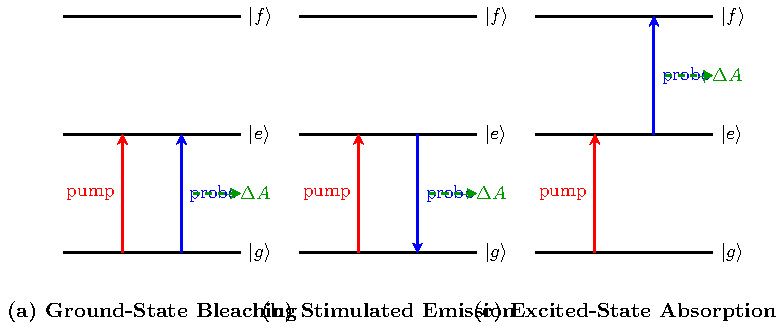
\includegraphics[width=0.9\textwidth]{chapters/figures/transient_absorption_pathways.pdf}
%    \caption{Schematic representation of the three primary contributions to transient absorption signals: (a) Ground-State Bleaching, (b) Stimulated Emission, and (c) Excited-State Absorption. Each pathway involves different transitions between the levels of a four-level system.}
%    \label{fig:transient_absorption_pathways}
%\end{figure}

\noindent Figure \todoref{include and ref the figure} illustrates these three primary contributions to transient absorption signals.

\noindent Analysis of these features as a function of time delay provides information about excited-state lifetimes, energy transfer processes, and photochemical reaction pathways. The ability to separate and identify these contributions is crucial for understanding the dynamics of complex molecular systems \todoref{find ref}%\cite{berera2009, megerle2009}.

%-------------------------------------------------------------------------------
%	SECTION 6: MULTIDIMENSIONAL SPECTROSCOPY APPLICATIONS
%-------------------------------------------------------------------------------

\iffalse
	\section{Multidimensional Spectroscopy in Structural Biology and Chemistry}
	\label{sec:multidimensional_applications}

	\subsection{Time- and Structure-Resolution Challenges}
	\label{subsec:time_structure_challenges}

	\noindent Scientific questions encompassing both the structure and dynamics of molecular systems present significant experimental challenges \cite{hammzanni2011conceptsmethods2d}. Consider fundamental processes such as protein folding, solvent fluctuations, or electron transfer reactions. In each case, researchers seek to understand the reaction pathway, which requires time-resolving the molecular structure. However, the relevant time scales can span an enormous range—from femtoseconds to hours—depending on the specific system under investigation.

	\noindent Traditional spectroscopic methods face inherent limitations in simultaneously achieving high temporal and structural resolution. When dynamics occur on slow time scales, nuclear magnetic resonance (NMR) spectroscopy can provide exquisite structural information with atomic-level detail. Conversely, for fast processes, fluorescence or absorption spectroscopy can probe dynamics with exceptional temporal resolution, but with a corresponding trade-off in structural specificity \cite{hammzanni2011conceptsmethods2d}. Between these extremes lies an experimental gap in both time- and structure-resolution capabilities.

	\noindent This gap becomes even more pronounced when studying dynamics in confined environments such as biological membranes, where many standard structural techniques become difficult or impossible to apply. The challenge is particularly acute for intermediate time scales (picoseconds to microseconds) and for systems where both structural changes and dynamic processes are coupled.

	\subsection{2D IR Spectroscopy: Bridging the Gap}
	\label{subsec:2dir_bridging_gap}

	\noindent Two-dimensional infrared (2D IR) spectroscopy has emerged as a powerful technique to address these limitations, providing bond-specific structural resolution across all relevant time scales \cite{hammzanni2011conceptsmethods2d}. This technique offers several unique advantages:

	\begin{itemize}
		\item \textbf{Temporal versatility:} 2D IR spectroscopy possesses the fast time resolution necessary to follow electron transfer and solvent dynamics on femtosecond time scales, while also being applicable in "snapshot" mode to study kinetics extending to arbitrarily long time scales.

		\item \textbf{Sample flexibility:} The technique can be applied to diverse sample types, including dilute solutions, solid-state systems, and membrane-bound proteins, making it particularly valuable for biological applications.

		\item \textbf{Structural sensitivity:} The method derives its structural information from couplings between vibrational modes that give rise to characteristic infrared bands and cross-peaks. These cross-peaks provide direct information about molecular connectivity and conformational changes.

		\item \textbf{Environmental probes:} Molecular structures can be probed through hydrogen bonding patterns and electric field effects that generate dynamic 2D lineshapes, providing insights into local environments and intermolecular interactions.
	\end{itemize}

	\noindent The structural sensitivity of 2D IR spectroscopy stems from the fact that vibrational frequencies are exquisitely sensitive to local molecular environment, hydrogen bonding, and electrostatic interactions. Cross-peaks in 2D IR spectra arise from vibrational coupling and provide direct information about spatial proximity and connectivity between different molecular groups \cite{hammzanni2011conceptsmethods2d}.

	\subsection{Computational Integration and Future Directions}
	\label{subsec:computational_integration}

	\noindent A particularly powerful aspect of 2D IR spectroscopy is that the spectra can be quantitively computed from molecular dynamics simulations, providing a direct comparison between experimental observations and all-atom theoretical models \cite{hammzanni2011conceptsmethods2d}. This computational-experimental synergy enables:

	\begin{itemize}
		\item Validation of molecular dynamics force fields and simulation protocols
		\item Assignment of spectral features to specific molecular structures and conformations
		\item Prediction of spectroscopic signatures for proposed molecular mechanisms
		\item Development of structure-spectrum relationships for complex systems
	\end{itemize}

	\noindent While 2D IR spectroscopy can be used qualitatively as an analytical tool, a deeper understanding of nonlinear optics, vibrational potentials, and lineshape theory enables much more sophisticated interpretation of 2D spectra and expands the range of possible applications \cite{hammzanni2011conceptsmethods2d}.

	\noindent The principles and methods developed for 2D IR spectroscopy also extend to 2D visible spectroscopy, which probes electronic transitions and has found particular application in studying photosynthetic light-harvesting complexes and other photobiological systems. Looking toward the future, pulse sequences for three-dimensional (and higher-dimensional) spectroscopy are being developed, promising even greater structural and dynamical information content \cite{hammzanni2011conceptsmethods2d}.

	\noindent The integration of multidimensional spectroscopic techniques with advanced computational methods represents a paradigm shift in how complex molecular systems can be studied, offering unprecedented insights into the relationship between molecular structure, dynamics, and function.

	%----------------------------------------------------------------------------------------
	%	CONCLUSION
	%----------------------------------------------------------------------------------------

	\section{Summary and Outlook}
	\label{sec:summary}

	\noindent Spectroscopy continues to evolve as a cornerstone analytical technique in physical sciences \cite{mukamel1995principlesnonlinearoptical, cho2009twodimensionalopticalspectroscopy}. From the basic principles of light-matter interaction to advanced nonlinear methods, spectroscopic approaches provide unique insights into the structure, dynamics, and function of complex systems across multiple time and length scales.

	\noindent Recent developments in laser technology, detection methods, and theoretical frameworks have expanded the frontiers of spectroscopy \cite{jonas2003twodimensionalfemtosecondspectroscopy} \todoref{find ref}%, Shim2009}.
	Attosecond spectroscopy now probes electron dynamics on their natural time scale, while quantum light sources open new possibilities for quantum-enhanced measurements.

	\noindent The integration of spectroscopic methods with imaging techniques, such as super-resolution microscopy and spectroscopic tomography, bridges the gap between molecular-level information and macroscopic observations \cite{brixneretal2004phasestabilizedtwodimensionalelectronic}.
	Meanwhile, the application of artificial intelligence and machine learning approaches to spectral data analysis promises to reveal subtle patterns and correlations that might otherwise remain hidden.

	\noindent As our understanding of light-matter interactions deepens and experimental capabilities advance, spectroscopy will continue to provide critical insights across chemistry, physics, biology, and materials science, contributing to technological innovations and fundamental scientific discoveries.


	\todoidea{ADD:TODO \\
		In real molecular systems, individual molecules don't have identical properties due to:

		Static Disorder: Different local environments cause each molecule to have slightly different transition frequencies
		Conformational Variations: Molecular geometry differences affect electronic transitions
		Solvent Effects: Local electric field variations from surrounding solvent molecules
		Sample Preparation: Manufacturing imperfections introduce site-to-site variations
		This creates inhomogeneous broadening - a distribution of transition frequencies (typically Gaussian) around a central value. To simulate realistic spectra that match experiments, you must:

	}
\fi